%max: 5pages

\documentclass{llncs}
%
\usepackage{makeidx}  % allows for indexgeneration
\usepackage{graphicx} % for photos
%
\begin{document}
%
\frontmatter          % for the preliminaries
%
\pagestyle{headings}  % switches on printing of running heads
\addtocmark{Hamiltonian Mechanics} % additional mark in the TOC
%

\mainmatter              % start of the contributions
%
\title{Zone-project: towards a better news feed using semantic web}
%
\titlerunning{Zone-project}  % abbreviated title (for running head)
%                                     also used for the TOC unless
%                                     \toctitle is used
%
\author{Christophe Desclaux\inst{1}}
%
\authorrunning{Christophe Desclaux} % abbreviated author list (for running head)
%
%%%% list of authors for the TOC (use if author list has to be modified)
\tocauthor{Christophe Desclaux}
%
\institute{Wimmics Inria, Sophia Antipolis...,\\
\email{christophe@zouig.org},\\ WWW home page:
\texttt{http://www.zone-project.org}
}

\maketitle

\begin{abstract}%
Nowadays we can use RSS feeds, Twitter, Google Reader, Yahoo Pipes or aggregators to keep up with news. However those solutions do not guarantee data privacy and usually manage news by origin. 
The zone project proposes an innovative solution to overcome those issues using the power of Semantic Web to group related informations together.
ZONE-project provides a new, innovative way to follow news. 
At its core, the system is aggregating news items from various RSS feeds.
Using semantic web we are able to efficiently tag and annotate each news. 
Those tags are the basis of filters to allow users to see only news that are relevant.


%The abstract should summarize the contents of the paper
%using at least 70 and at most 150 words. It will be set in 9-point
%font size and be inset 1.0 cm from the right and left margins.
%There will be two blank lines before and after the Abstract. \dots
\keywords{linked data, data aggregation, RSS}
\end{abstract}
%
\section{Motivation}
%
A lot of news are published every day on internet, the number of news websites has increased significantly. People and organizations are now building news aggregators in order to sort all this information. This systems are really important in order to clean all the amount of information.

Solutions exist, for instance one can use \textsl{Google news} \footnote{\url{http://news.google.fr}} like a trusted provider of information, but in this web application your are only a consumer and don't have a lot of interactions with the system. 

The second solution is to make news forecasting using \textsl{Twitter}\footnote{\url{http://www.twitter.com}}, it's a  solution in which one can control the sources he follows. But you can't have a selection on sources and on topics and you have a lot of noise around goods informations.
***************** oui, les recherches par mots tags ne permettent pas de supprimer les bruit liés à l'utilisation de mêmes hashtags sur différents sujets distincts **************************


The last relevant solution that one can use is \textsl{Yahoo Pipes} \footnote{\url{http://pipes.yahoo.com/pipes/}}, this tool allows the mixing of popular data feeds to create data filtering via a visual editor. It uses pipes as workflows which will help users to sort feeds.

From these three types of approaches we can identify some main challenges that good aggregators need to work on.
\begin{itemize}
  \item \textbf{filtering capacities} we need to be able to select and sort information according to precise criteria.
  \item \textbf{lots of informations} the tool needs to have access to a maximum of news present on internet 
  \item \textbf{privacy} users need to use the solution independently of any source provider.
\end{itemize}

Technicals solutions exists in order to solve this challenges, Google solve this problem using [article de Larry Page sur l'aggregation par mots clés] but this solution is not very efficient because it works on words instead of working on meaning. The solution we propose is an aggregation based on semantic web frameworks. 

We will first present in this article how our solution called Zone. We will explain the annotation workflow, the ontology used and the use of data-mining solutions. The we will present a demonstration of the application and finally conclude and talk about future work.

%
\section{Application: Zone}


\subsection{the workflow}
%
\begin{figure}[htb!]
	\begin{centering}
	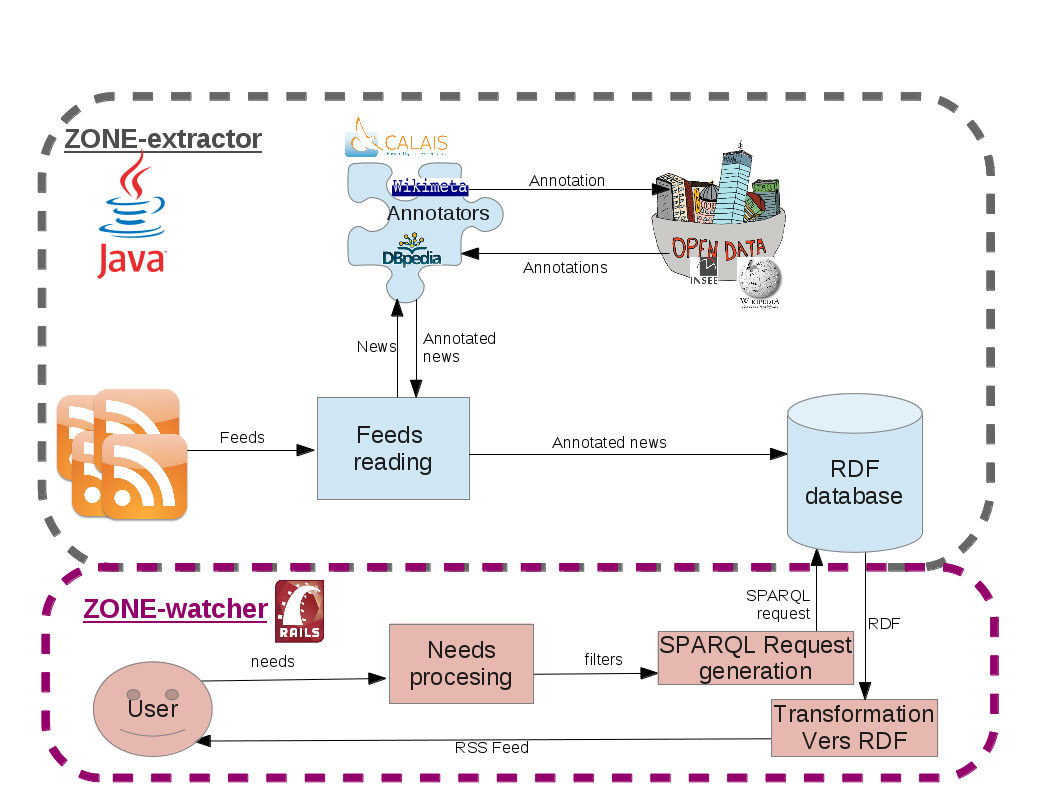
\includegraphics[width=1\textwidth]{diagramArchi.png}
	\caption{Workflows d'annotation et de filtrage sémantique de nouvelles}
	\label{fig:WF}
	\end{centering}
\end{figure}

In order to have a selection more efficient of news according to their semantic relevance, we have created two sort of workflows, figure \ref{fig:WF} shows the general architecture: a semantic annotation workflow of news and a filtering workflow. The distinction between the two workflows is extremely important in order to work in an asynchronous way.




\subsubsection{The semantic annotation workflow}
He crawled the web extracting all news and storing them in database next to semantic annotations.
In order to make the news retreival we use RSS feeds technologies and will not present them in details. The storage of the news is made 
We will present more in details the annotation procesus and the use of links with linkedOpenDatas, for the news retreival we ue techno

%\subsubsubsection{Annotators}
********************citer les différents et comment ils marchent et aussi le ExtractArticleContent********************

\subsubsection{The filtering workflow}
He is giving the user the possibility to access all datas organized by the annotation workflow. He is organized as a web application using the web framework RubyOnRails \footnote{\url{http://rubyonrails.org}} which help us to build the web application. In order to create the SPARQL requests on database we ask with examples to the user which annotations he want to follow. He can make some tests of filters on the website in order to see what will be the result of the filter. Last he can create a RSS feed based on this filters.
%
\subsection{The ontologie}
%
**************basée sur RSS
on a ajouté un schéma RDFs spécialisé
on se base aussi sur l'ontologie de wikimeta/insee***************
%

%
\subsection{Using generalisators}
*******parler de l'insee********

%
\subsection{Using datamining}
section d'Ameni

\section{Demonstration}
%
The web application is designed for all kind of news feed like technological, medical or general news feed. You can install the application according to your needs and the AGPL licence. We also propose a web application for general news feed on \url{http://demo.zone-project.org} which is the main test platform for the application.

The demo starts with the listing of all recent news on \url{http://demo.zone-project.org}. Then we create a filter according to some criteria in order to show to the audience the different kind of filters present and their links to the news. Finally, when the good filter is chosen, we export it to an external RSS feed aggregator showing that our web application can be use in combination of other tools.

Then we propose an other usage of ZONE-project, according to twitter. We go on the demo application and make a quick demonstration of news filtering on the hashtag #eswc2013.

\section{Conclusion and futur work}
%
Challenges qui restent à résoudre :
	*tech : faire des liens vers openData et du raisoning
	*com : trouver moyen de pérenniser le projet
%

\section{Acknowledgments}
%
This project has been started in 2011 according to an and of ingeneering school project and has been 
Description du contexte de travail=> se passe à l'inria BYC... équipe wimmics qui bosse sur semantic web

%





%
% ---- Bibliography ----
%
\begin{thebibliography}{5}
%
\bibitem {clar:eke}
Clarke, F., Ekeland, I.:
Nonlinear oscillations and
boundary-value problems for Hamiltonian systems.
Arch. Rat. Mech. Anal. 78, 315--333 (1982)

\bibitem {clar:eke:2}
Clarke, F., Ekeland, I.:
Solutions p\'{e}riodiques, du
p\'{e}riode donn\'{e}e, des \'{e}quations hamiltoniennes.
Note CRAS Paris 287, 1013--1015 (1978)

\bibitem {mich:tar}
Michalek, R., Tarantello, G.:
Subharmonic solutions with prescribed minimal
period for nonautonomous Hamiltonian systems.
J. Diff. Eq. 72, 28--55 (1988)

\bibitem {tar}
Tarantello, G.:
Subharmonic solutions for Hamiltonian
systems via a $\bbbz_{p}$ pseudoindex theory.
Annali di Matematica Pura (to appear)

\bibitem {rab}
Rabinowitz, P.:
On subharmonic solutions of a Hamiltonian system.
Comm. Pure Appl. Math. 33, 609--633 (1980)

\end{thebibliography}

\clearpage
\end{document}